\chapter{Az alkalmazás}
\section{Architektúrális felépítés}
A webshop program három fő résszel rendelkezik. Egy frontend, amit a felhasználó a böngészőből elér; egy backend, amivel a frontend kommunikál; ez pedig egy adatbázisból nyeri ki a termékek adatait. A frontend-backend kommunikáció HTTP-n keresztül történik, a chat funkcionalitás pedig WebSocket segítségével. A backend TCP kapcsolaton keresztül éri el az adatbázist.
\vskip 0.1in
\textit{Megjegyzés: az alkalmazás használt protokollokra a 2.1.3-as fejezetben részletesen kitérek.}
\begin{figure}[ht]
\centering
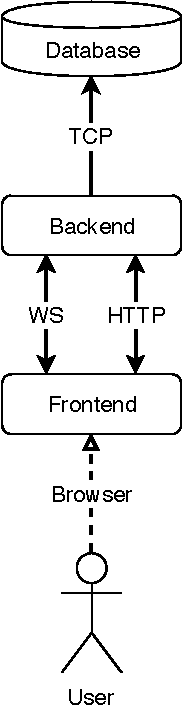
\includegraphics[width=24mm, keepaspectratio]{img/app_architecture.pdf}
\caption{A példa alkalmazás felépítése.}
\end{figure}
\vskip 0.1in
\newpage
\subsection{Frontend}
A webalkalmazás "látható" részét a frontend teszi ki. Reactban íródott ami egy JavaScript alapú web keretrendszer: a FaceBook hozta létre, és felhasználói felületek építésére használják.\cite{Node_W3} Mivel JavaScript alapú, így a programkód npm\footnote{Node Package Manager - \url{https://www.npmjs.com/}} segítségével fordítható.

A felület lehetőséget nyújt termékkategóriák böngészésére (ez a menüben dinamikusan generált), és ott termékek kosárba helyezésére. Továbbá chatelhetünk is az oldalon tartózkodó egyéb felhasználókkal.

\begin{figure}[ht]
\centering
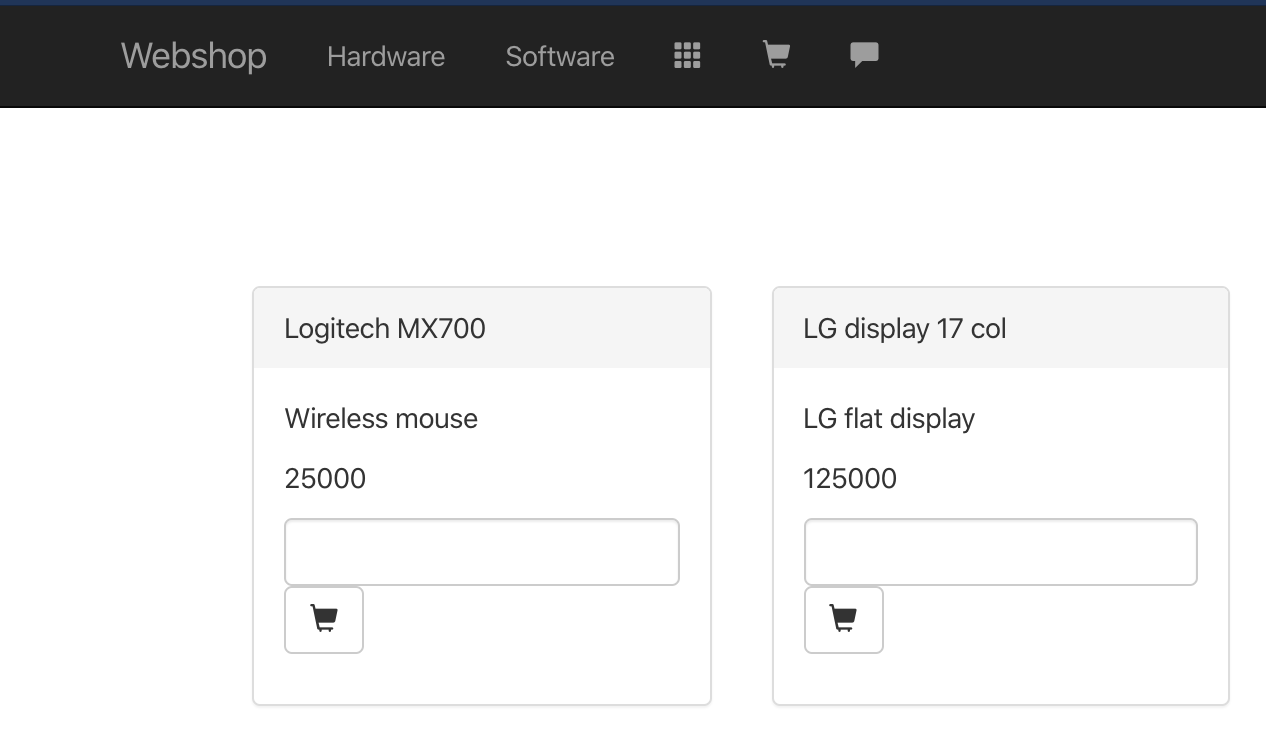
\includegraphics[width=150mm, keepaspectratio]{img/frontend.png}
\caption{Az alkalmazás kinézete.}
\end{figure}
\subsection{Backend}
A backend egy Springben íródott program. Ez egy Java alapú alkalmazás keretrendszer, mely 2003 óta létezik és jelenleg is aktív fejlesztés alatt ál. A futtathatóságot jelentősen leegyszerűsítendő, az alkalmazás Spring Boot-ot használ mely lényegében azt teszi lehetővé, hogy egy Springben írt alkalmazás \textit{click-to-run} (azaz egy kattintással futtatható) legyen.\cite{SpringBoot}

A program futtatáshoz le kell töltenünk a szükséges függőségeket és azt az alkalmazással együtt csomagolni. A backend készítői Maven buildkezelőt használnak, ami többek között a fenti feladatokat is ellátja.
\subsubsection{Adatbázis}
Az alkamazás a termékek listáját egy adatbázisból olvassa ki. Erre Postgres-t használ, egészen pontosan annak 11-es verzióját.
\vskip 0.1in
\textit{Megjegyzés: a használt adatbázismotor később lett Postgresre cserélve, mert a skálázás megvalósításához ez elkerülhetetlen volt. Eredetileg HyperSQL\footnote{Javaban írt adatbázismotor - \url{http://hsqldb.org/}} volt használva, azonban az a skálázáshoz létszükéges replikációt\footnote{Adatbázisok közti adatok szinkronizálása} nem támogatta.\cite{HSQL}}

Jelenleg két tábla létezik, az egyik a kategóriákat, míg a másik az azokba tartozó termékeket tárolja, ahogyan az az éles rendszerből lekért adatokon látszik:
\begin{lstlisting}
webshop=# \dt
          List of relations
 Schema |   Name   | Type  |  Owner
--------+----------+-------+----------
 public | category | table | postgres
 public | product  | table | postgres
(2 rows)

webshop=# select * from category;
 id |   name
----+----------
  1 | Hardware
  2 | Software
(2 rows)

webshop=# select * from product;
 id |          description           |          name           | price  | category_id
----+--------------------------------+-------------------------+--------+-------------
  1 | Wireless mouse                 | Logitech MX700          |  25000 |           1
  2 | LG flat display                | LG display 17 col       | 125000 |           1
  3 | Laser pointer and presenter    | Microsoft laser pointer |   6800 |           1
  4 | The best office suite for home | Ms Office 2018 Home     |  25000 |           2
  5 | Graphical editing software     | Adobe Photoshop         | 125000 |           2
(5 rows)
\end{lstlisting}
\subsection{Kommunikáció a rétegek közt}
Ahogyan az a 2.1-es ábrán látszik, három fő kommunikációs csatorna valósul meg a rétegek közt:
\begin{enumerate}
    \item Adatbázis <--> Backend: TCP\footnote{Transfer Control Protocol} segítségével történik az adatok lekérése. A backend JDBC Drivert\footnote{Java DataBase Connectivity API - Olyan Java komponens mely lehetővé teszi az adatbázissal való kommunikációt} használ, és a megalkotott SQL utasításokat elküldi az adatbázisnak, aki arra válaszul visszaküldi az eredményt.
    \item Backend <--> Frontend: HTTP segítéségvel, egy API végponthoz fordulva történik az adatok lekérése. Úgy kell elképzelni, hogy a frontend betöltésekor kapunk egy leírót, hogy hogyan néz ki az oldal, és hol van az adatok helye. De azoknak lekérése nem a frontend dolga, pusztán azt mondja meg hol találjuk azt. Ezek után a felhasználó böngészője már az backendhez fordul.
    \vskip 0.1in
    \textit{Megjegyzés: azért nem közvetlenül az adatbázishoz kapcsolódik a kliens mert ez nem biztonságos, például közvetlenül ki lehetne olvasni az adatbázistábla szerkezetét és akár olyan adatokat is, melyeket nem lenne szabad. A másik ok pedig, hogy így könnyen válthatunk adatbázismotort, hisz csak a backendet (sőt, ott is csak a JDBC drivert) kell cserélni.}
    \item Backend <--> Frontend: WebSocket segítségével zajlik a kommunikáció. Bár lentebb kifejtem részletesen, de röviden: a chat funkcionalitás megvalósítása miatt szükséges ezen protokoll bevezetése, hogy valós idejű kommunikáció jöhessen létre a szerver és kliens között.         
\end{enumerate}
\newpage
\subsubsection{HTTP}
\textbf{HyperText Transfer Protocol - a web alapja}

Bár a szakdolgozatom témájához szorosan nem kapcsolódik, mégis érdemesnek tartom ezt a féloldalas kitérőt a HTTP protokoll felé, hiszen a ma ismert web magjának részét képzi. Egy 24 éves alkalmazásbeli (\textit{7. rétegbeli}) protokollról beszélünk, mely a mai napig fejlesztés alatt áll: első verziója a HTTP/1.0 volt, (sajnos) jelenleg legelterjedtebb változata a HTTP/1.1\cite{ripHTTP2}, illetve 2015-ben jelent meg a modernnek számító HTTP/2.0\cite{HTTP2_RFC}

A könnyebb megértés érdekében szeretném részletezni a HTTP/1.1 protokollt.

Három alapvető részből épül fel:
\begin{itemize}
    \item \textbf{request line}
    \item \textbf{request body}
    \item \textbf{message body}
\end{itemize}
Talán a \textit{request line} a legfontosabb, mely két részből épül fel: egy kérés típusból illetve egy útvonalból melyhez a kérést intézzük. Az alábbi kéréstípusok léteznek:
\begin{itemize}
    \item \textbf{GET} - az erőforrás elérése, lekérdezése.
    \item \textbf{HEAD} - hasonló a GET metódushoz, azonban csak a fejlécet kérdezi le.
    \item \textbf{POST} - az elérni kívánt útvonaltól a \textit{message body}ban található adatok feldolgozását kérelmezi.
    \item \textbf{PUT} - hasonló a POST metódushoz, azonban feldolgozás helyett pusztán tárolást kér.
    \item \textbf{PATCH} - hasonló a PUT metódushoz, azonban ez csak a szolgáltatott adatokat írja felül, nem új bejegyzést hoz létre.
    \item \textbf{DELETE} - adatok törlését kérelmezi a kiszolgálótól.
    \item \textbf{TRACE} - a kiszolgáló válaszul a beérkezett HTTP kérést küldi vissza.
    \item \textbf{OPTIONS} - az elérhető HTTP metódusok lekérdezésére szolgál.
    \item \textbf{CONNECT} - TCP kapcsolat felépítésére ad lehetőséget.
\end{itemize}

A kiszolgáló válaszul szintén egy három részes csomagot küld.
\begin{itemize}
    \item \textbf{response status line}
    \item \textbf{response header}
    \item \textbf{message body}
\end{itemize}
Szintén az első részt szeretném részletezni, ugyanis hibakeresésekhez rendkívül hasznos. Ez három alrészből áll: HTTP verzió, HTTP státuszkód, rövid leírás a státusszal kapcsolatban. A státuszkódot az alábbi öt kategóriába lehet sorolni:
\begin{itemize}
    \item \textbf{1xx} - információ közlése
    \item \textbf{2xx} - sikeres művelet \textit{(Gyakorlati példa: HTTP200 - OK)}
    \item \textbf{3xx} - átirányítás
    \item \textbf{4xx} - kliensoldali hiba \textit{(Gyakorlati példa: HTTP404 - NOT FOUND)}
    \item \textbf{5xx} - szerveroldali hiba
\end{itemize}

\subsubsection{WebSocket}
A WebSocket protokoll kétirányú kommunikációt tesz lehetővé a kliens és a távoli kiszolgáló között. A kommunikáció megkezdése egy nyitó kézfogásból és egy egyszerű üzenetből áll, TCP felett. A protokoll célja, hogy a kliens és szerver közti kétirányú kommunikáció meg tudjon valósulni több HTTP kapcsolat létrehozása nélkül (ami egyébként RFC szerint sérti is a HTTP/1.1 szabányt\cite{HTTP_RFC})\cite{WS_RFC}.

Gyakori tévedés, hogy a WebSocket bármilyen formában is függ a HTTP protokolltól. Két megtévesztő tulajdonságot figyelhetünk meg ami erre okot adhat. Alapértelmezetten a WebSocket is 80-as porton kommunikál a HTTP-hez hasonlóan, illetve a TLS\footnote{Transport Layer Security} feletti, biztonságos változata is a 443-as porton (WebSocket Secure, HyperText Transfer Protocol Secure). A másik ok pedig az, hogy a kezdeti kézfogás egy HTTP Upgrade kérelemként jelenik meg a webkiszolgáló számára.
A WebSocket URI\footnote{Uniform Resource Identifier}-ja a következőképp néz ki:
\begin{itemize}
    \item Nem-biztonságos kapcsolat definiálása esetén: \lstinline{ws://}
    \item Biztonságos, TLS feletti kapcsolat kérése esetén: \lstinline{wss://}
\end{itemize}

\textbf{A példaalkalmazás természetesen biztonságos kapcsolatot fog használni mind WebSocket, mind HTTP kommunikációra.}
\section{A hagyományos megközelítés}
Ebben a fejezetben azt szeretném megmutatni, hogy milyen lenne az alkalmazás fejlesztése és üzemeletetése, ha nem használnánk azokat a technikákat, technológiákat amikről egyébként a dolgozatom szól.
\subsection{Fejlesztés}
Ahogy azt az 1.1.1.1-es fejezetben már bemutattam, \textit{Continuous Integration} nélkül nem gördülékeny a fejlesztés. A csapatoknak magasszintű kooperációra van szükségük, ezáltal értékes mérnökórák vesznének el a fejlesztők (vagy a csapaton belüli emberek) koordinálására. Tehát legjobb esetben is azt feltételezhetjük, hogy a fejlesztés során verziókezelt kódbázissal dolgoznak.
\subsubsection{Tesztelés}
A tesztelésnél sajnos már korántsem biztos, hogy élnék azzal a feltételezéssel, hogy egyáltalán van átfogó tesztelés a szoftverfejlesztés ciklusában. Tegyük fel, létezik ilyen, vannak a programhoz készült tesztesetek. Ekkor ezt célszerű lenne minden programkód-kiadás előtt lefuttatni. De ez ismételten az automatizálás hiányából eredő időkidobás lenne. 
\subsubsection{Alkalmazásfrissítés}
Tételezzük fel, hogy a tesztelt webalkalmazás összes szükséges eleme rendelkezésünkre áll. Rosszabb esetben egyszerre kellene három komponenst cserélnünk. Mivel nem automatizált a módszer így ez időt vehet igénybe (és ismét értékes mérnökórák vesznek el...), de még vállalható lenne, és webalkalmazás esetén minimális (de nem nulla idejű) kieséssel járna. Viszont tegyük fel, hogy az alkalmazásból több példány fut egyszerre. Ez már kezelhetetlen lenne, hatékonyabb megoldás szükséges.
\subsection{Üzemeltetés}
Egy ilyen webalkalmazás üzemeltetésére többféle infrastruktúrát / megoldást lehete alkalmazni, mindegyiknek van előnye és hátránya is. Több dologra érdemes figyelni: költséghatékonyság, üzembiztonság, karbantarthatóság.
\subsubsection{Infrastruktúrális áttekintés}
A legegyszerűbb megoldás: mindent egy szerverre telepíteni és készen is vagyunk. Egy számítógépet kell venni, valószínűleg egy ideig az erőforráskihasználtság is optimális szinten lesz, mégis talán ez a legrosszabb megoldás. Mi történik akkor ha az eszköz meghibásodik? Szolgáltatáskieséssel kell számolnunk, mégpedig nem is röviddel. Csinálhatjuk azt is, hogy több kiszolgálót veszünk és mindenki a maga feladatát látja el (egy kiszolgáló - egy alkalmazáskomponens). Ez talán mégrosszabb gondolat, mert háromszoros lesz a meghibásodás esélye. Valami olyan megoldás kellene ami magasabb rendelkezésreállást tud nyújtani. Csinálhatunk egy klasztert\footnote{Összefűzött számítógépek, melyek egységnek tekinthetőek}, tehát több gépre telepítjük fel az alkalmazás mindhárom komponensét és ezeket egy terheléselosztó (\textit{Load-Balancer}) mögé helyezzük, ezzel biztosítva azt, hogy egy kiszolgáló (vagy alkalmazás) meghibásodása esetén még szolgáltatni tudunk.

Egy költséghatékonyabb és izoláltabb (biztonságosabb) megoldást jelenthet a \textit{virtualizáció} alkalmazása, ahol a fizikai számítógépek gyakorlatilag virtualizált környezetben (számítógépeken) futtatnak operációs rendszert, amire aztán az alkalmazáskomponensek telepíthetőek. Így például változó erőforrásméretű gépeket is költséghatékonyan ki tudunk használni (értsd: mondjuk kétszer annyi komponens az "erősebb" kiszolgálón).